\chapter[Scarefault]{Scarefault}
Neste capítulo, será abordado o \Scarefault, o produto final desse
trabalho. Este capítulo está dividido em seções. A primeira seção aborda
uma visão geral do \Scarefault. A segunda seção faz uma análise da
arquitetura do \framework e suas dependências. Na seção seguinte, explana-se
a respeito da utilização do \Scarefault.

\section{\Scarefault: Visão Geral}
O \scarefault é um \framework que tem a intenção de gerar testes unitários
de forma semiautomatizada. Para isso, ele necessita da intervenção do
desenvolvedor que o utiliza por meio de breves especificações nos
comentários de documentação. A partir dessas especificações, o \scarefault
coleta informações necessárias para a produção dos casos de teste e gera
um arquivo contendo os testes solicitados. É importante ressaltar que,
para esse trabalho, os testes gerados são apenas testes caixa preta.

O \framework propõe-se em permitir a acoplagem de diferentes linguagens
de programação. Para isso, há a necessidade da construção de um \parser
que identifique a sintaxe da linguagem alvo por meio de duas
ferramentas: \flexcpp e \textsf{Bisonc++}. Essas duas ferramentas são
comuns em contextos de produção de compiladores. Com o \parser
implementando, o desenvolvedor pode implementar as especificidades
relacionadas aos testes da linguagem alvo, tendo como base o código
oferecido pelo \Scarefault.

O \scarefault foi escrito em \textsf{C++}, e está licenciado dentro das condições
da \textsf{GPLv3}. Todo o código fonte desse framework encontra-se em:
\url{https://github.com/Scarefault/scarefault}.

\section{A Arquitetura do \scarefault} \label{sec-arq-scarefault}
Essa seção evidencia os elementos da arquitetura do \Scarefault. Como
ele foi desenhado, quais conceitos foram utilizados, e como ele funciona.
Em um primeiro momento, são exploradas visões estáticas da arquitetura.
A visão dinâmica da arquitetura é evidenciada pela seção \ref{sec-util-scarefault}.

\subsection{Visão de Pacotes}
Partindo-se de uma visão macroscópica, o \scarefault pode ser dividido em
dois módulos básicos: o \textit{identifier} e o \textit{generator}. A Figura
\ref{modules-scarefault} ilustra esses módulos básicos.

\begin{figure}[h]
  \centering
    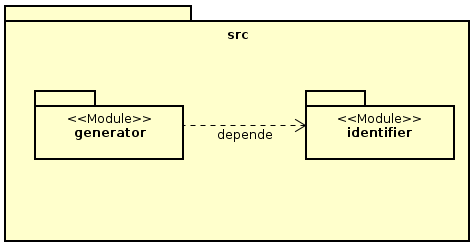
\includegraphics[width=0.6\textwidth]{figuras/modules-scarefault.png}
    \caption{Representação dos módulos do \scarefault}
    \label{modules-scarefault}
\end{figure}
\FloatBarrier

\begin{description}
\item[\textit{identifier}:] é responsável pela identificação das regras que regem
a gramática da linguagem de programação alvo, bem como pela coleta dos dados
necessários para a produção dos casos de teste.
\item[\textit{generator}:] responsável pela geração dos casos de teste. A partir dos dados
coletados das especificações do desenvolvedor e do próprio código fonte, esse
módulo é capaz de gerar casos de teste.
\end{description}

Expandindo-se os módulos, podem ser observados os pacotes associados a cada um deles,
e o relacionamento entre esses pacotes, como mostra a Figura
\ref{expand-modules-scarefault-1}.

\begin{figure}[h]
  \centering
    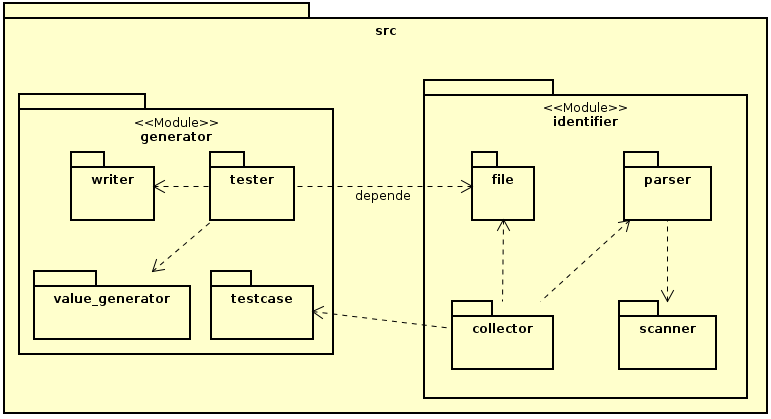
\includegraphics[width=0.8\textwidth]{figuras/expand-modules-scarefault-1.png}
    \caption{Representação expandida dos módulos do \scarefault}
    \label{expand-modules-scarefault-1}
\end{figure}

Como indicado na Figura \ref{expand-modules-scarefault-1}, os pacotes associados ao
módulo \textit{identifier} são:
\begin{description}
\item[\textit{scanner}:] responsável pela análise léxica do arquivo contendo o código
fonte em avaliação. As classes contidas nesse pacote são geradas pelo \flexcpp durante
a compilação.
\item[\textit{parser}:] responsável pela análise sintática do arquivo contendo o
código em avaliação. As ações que ele executa quando determinada regra gramatical é
encontrada são, essencialmente, ações de coleta de dados. As classes associadas
a esse pacote são geradas pelo \bisoncpp durante a compilação.
\item[\textit{collector}:] responsável pela coleta de dados necessários para a
criação de testes unitários.
\item[\textit{file}:] responsável por guardar os dados coletados do código fonte.
Dados esses, tais como as dependências (\textit{libraries} importadas), métodos e classe
do arquivo em análise.
\end{description}

Os pacotes associados ao módulo \textit{generator}, como mostra a Figura
\ref{expand-modules-scarefault-1}, são:
\begin{description}
\item[	\textit{tester}:] responsável pela construção dos arquivos de teste. A partir
dele é que os testes ganham forma, conforme a linguagem de programação.
\item[	\textit{testecase}:] responsável por guardar os dados relacionados
a cada caso de teste especificado pelo desenvolvedor, a partir dos
comentários no código fonte.
\item[	\textit{value\_generator}:] responsável por gerar valores randômicos
para o desenvolvimento dos testes.
\item[\textit{writer}:] responsável por escrever as informações do arquivo de
teste, enviadas pelo \textit{tester}. Para isso, ele cria o arquivo e
escreve todas as informações a ele solicitadas.
\end{description}

\subsection{Visão de Classes}
As Figuras \ref{modules-scarefault} e \ref{expand-modules-scarefault-1} mostram
a visão de pacotes do \scarefault e como eles se relacionam, bem como a
responsabilidade que cabe a cada um deles. Aprofundando-se mais, chega-se a uma
visão das entidades associadas a cada pacote. A visão de quais são essas
entidades e como elas se relacionam pode ser verificada pelo Modelo de 
Domínio, mostrado na Figura \ref{domain-diagram}.
\begin{figure}[h]
  \centering
    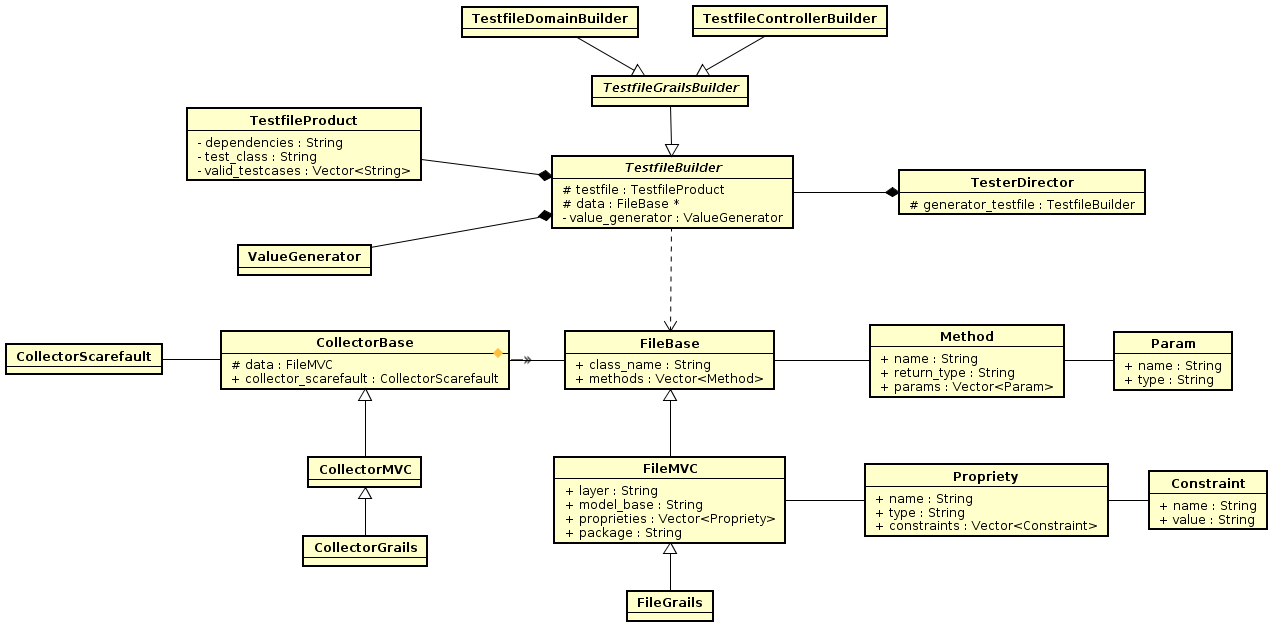
\includegraphics[width=\textwidth]{figuras/domain-diagram.png}
    \caption{Diagrama de domínio do \scarefault}
    \label{domain-diagram}
\end{figure}
\FloatBarrier

O modelo de domínio na Figura \ref{domain-diagram} demonstra a relação
entre as principais entidades que o \framework trabalha. O \textit{Collector}
recolhe as  informações essencias para os testes a partir do
\textit{Parser} que, por sua vez, recebe um \textit{stream} de dados a partir
do \textit{Scanner}. Como dados importantes para a produção de testes pelo
\Scarefault, tem-se métodos (\textit{Method}) e seus parâmetros (\textit{Param})
e, para arquiteturas voltadas ao MVC, tem-se propriedades (\textit{Propriety})
e suas restrições (\textit{Constraint}). Esses dados estão intimamente ligados
ao arquivo em análise, portanto, são armazenados na entidade arquivo (\textit{FileBase}).
Há também a entidade \textit{TestCase} que tem papel fundamental na produção
dos testes, pois carrega as informações dispostas pelo desenvolvedor sobre os
testes a serem criados. Uma parte importante dos casos de teste são os
argumentos (\textit{Arg}) que devem ser passados ao método em avaliação durante o
teste.

Partindo-se do modelo de domínio exposto na Figura \ref{domain-diagram}, pode-se
visualizar o diagrama de classe, mostrado na Figura \ref{class-diagram}.

\begin{landscape}
\begin{figure}[h]
  \centering
    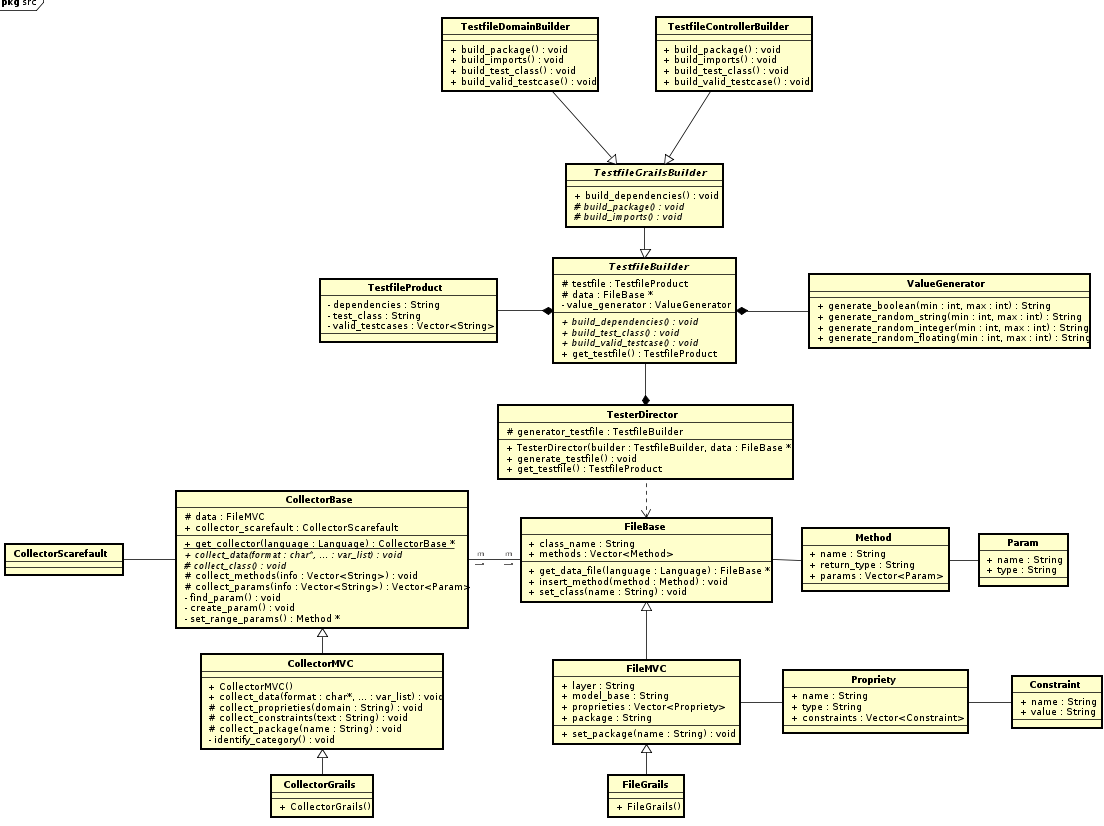
\includegraphics[width=1.5\textwidth]{figuras/class-diagram.png}
    \caption{Diagrama de classe completo do \scarefault}
    \label{class-diagram}
\end{figure}
\FloatBarrier
\end{landscape}

O diagrama de classes permite obter uma visualização mais apurada dos
relacionamentos entre as classes contidas no \textit{framework}. As principais
entidades do \textit{framework}, apresentadas na Figura \ref{domain-diagram},
estão presentes e muitas delas passaram a ter um conjunto auxiliar de classes,
de forma a permitir a sua adaptação ao contexto em que será inserida.

Por meio da Figura \ref{class-diagram}, pode-se identificar o uso de alguns
\textit{design patterns} de criação, com o intuito de permitir a
extensibilidade do \framework e a sua facilidade de uso. Para esse fim,
foram usados os conceitos do \textbf{\textit{builder pattern}} e
\textbf{\textit{factory pattern}}.

\subsubsection{\textit{Builder Pattern}}
O uso do \textit{builder pattern} procurou colaborar com a criação de objetos complexos. Seu intuito é a separação do processo
de construção da representação em si. Desse modo, é possível que o
mesmo processo de construção sirva para diferentes representações
\cite{gammaEtAl1994}.

No desenvolvimento do \textit{framework}, observou-se essa necessidade na
criação de objetos \lstinline|Testfile|. Essa entidade é diferente para
cada linguagem associada a ele. Não é possível manter uma mesma
representação desse objeto, no entanto, o processo de criação de um
\lstinline|Testfile| é igual em todos os casos: escreve-se as
dependências da classe de teste, o cabeçalho da classe de teste,
as ações iniciais para os testes (\textit{setup}),
os casos de teste, as ações para depois de cada teste
(\textit{teardown}) e a finalização do arquivo.

Nesse sentido, viu-se a solução proposta pelo \textit{builder pattern}
como saída para o problema dentro do contexto do desenvolvimento do
\Scarefault. A Figura \ref{testfile-diagram} mostra como a solução
foi desenhada.

%Ver comentário
\begin{figure}[h]
  \centering
    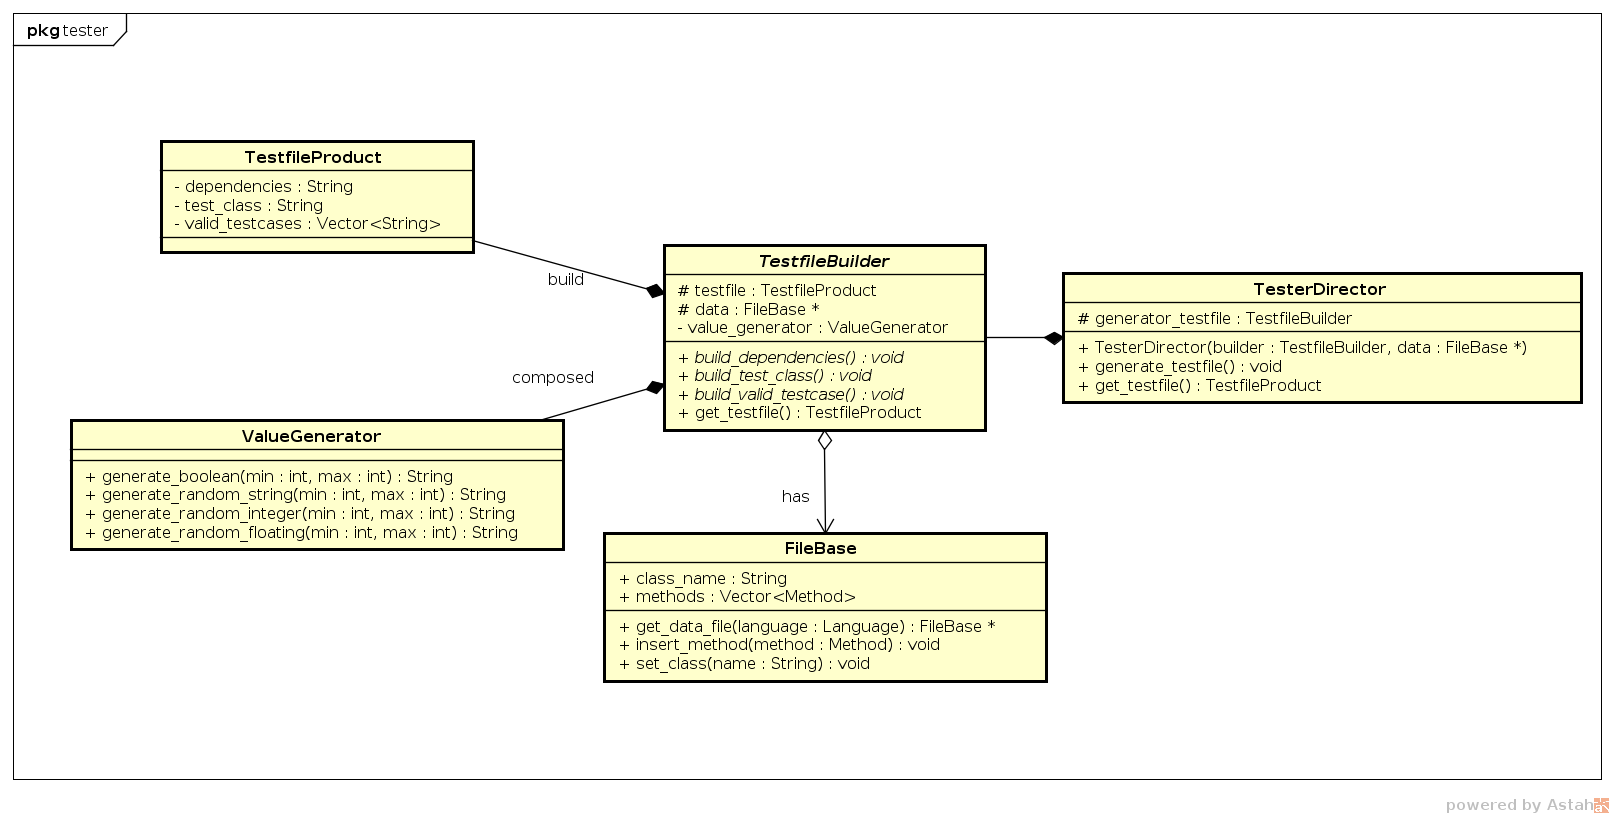
\includegraphics[width=\textwidth]{figuras/testfile-diagram.png}
    \caption{Diagrama de classes apresentando o \textit{builder pattern} no \framework}
    \label{testfile-diagram}
\end{figure}
\FloatBarrier

O objeto a ser construído é da classe \lstinline|TestfileProduct|. Há
diversas representações que esse objeto pode tomar, conforme a linguagem.
No entanto, o processo de construção é o mesmo. Os passos desse processo são definidos
pela classe \lstinline|TestfileBuilder|. Essa classe é uma classe
\lstinline|virtual| (abstrata). Ela define uma interface que deve ser
implementada pelas suas classes filhas, afim de construir o objeto
\lstinline|TestfileProduct|. Dessa forma, garante-se que qualquer
classe com a responsabilidade de construir um \lstinline|TestfileProduct|
terá funções-membro que criem os elementos essenciais do produto. Com a garantia
que os passos de construção estão implementados, pode-se fazer o processo de
criação. Essa atividade é responsabilidade do \lstinline|TestfileDirector|. O
método \lstinline|generate_testfile()| possui a definição do processo de
construção, a partir dos passos estipulados pelo \lstinline|TestfileBuilder|.

\subsubsection{\textit{Factory Pattern}} \label{subsec-factory-pattern}
\textit{Factory pattern} é uma solução pensada com o propósito de deixar a
instanciação de objetos de uma mesma família mais flexível. Através desse
padrão,  é possível instanciar um objeto sem expor a lógica dessa ação, bem
como ser capaz de referenciar-se a novos objetos por uma interface comum
\cite{gammaEtAl1994}.

No construção do \scarefault, deparou-se com a necessidade de flexibilizar
a instanciação de objetos de coleta de dados. Isso fornece maior liberdade
ao desenvolvedor usuário do \framework para criar suas próprias classes de
coleta, que estarão relacionadas a uma determinada linguagem de programação
e suas peculiaridades.

Por esse motivo, foi pensado no \textit{Factory pattern} como solução. A Figura
\ref{collector-diagram} mostra a solução desenhada para o \textit{framework}.

%%ver comentário

\begin{figure}[h]
  \centering
    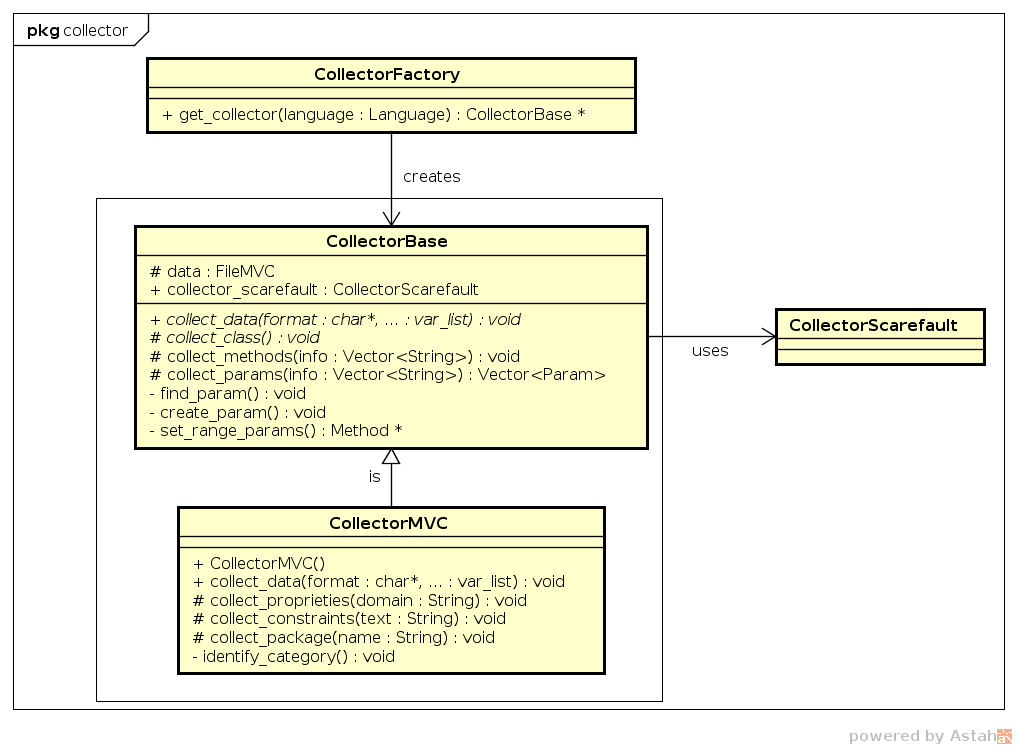
\includegraphics[width=\textwidth]{figuras/collector-diagram.png}
    \caption{Diagrama de classes apresentando o \textit{factory pattern} no \framework}
    \label{collector-diagram}
\end{figure}
\FloatBarrier

A solução de \textit{Factory pattern} desenvolvida utiliza-se de uma classe
\lstinline|virtual| denominada \lstinline|CollectorBase|. Optou-se por uma classe
desse tipo, ao invés de uma \lstinline|virtual| pura (\textit{interface}), pois
imaginou-se em já deixar implementadas determinadas funções-membro auxiliares,
preparadas para serem usadas pelo usuário. Essas funções-membro, embora já implementadas,
são passíveis de sobreescrita, o que dá a possibilidade do desenvolvedor
decidir criar as sua própria forma de coletar determinados elementos ou utilizar-se
de uma já disponível.

A única função-membro obrigatória de implementação para as classes derivadas da
\lstinline|CollectorBase| é a \lstinline|collect_data(char *, ...)|. Além disso, já
há uma outra classe de coleta preparada para linguagens que se utilizem do padrão
de projeto MVC: a \lstinline|CollectorMVC|. Ela também estende a \lstinline|CollectorBase|,
mas traz outras funções-membro auxiliares.

A classe \lstinline|CollectorFactory| é reponsável por esconder a lógica de instanciação
da família \textsf{Collector}. Por meio da \lstinline|get_collector()| um objeto
\lstinline|CollectorFactory| retorna uma instância do \textsf{Collector} solicitado na
classe cliente.

\section{A Utilização do \Scarefault} \label{sec-util-scarefault}
A seção \ref{sec-arq-scarefault} apresentou a visão estática da arquitetura do
\Scarefault. Nesta seção, pretende-se mostrar a visão dinâmica, por meio
de explicações a partir do uso do \textit{framework}. A utilização do
\scarefault pode ser dividida em dois objetivos: a adaptação
do \textit{framework} para atender uma nova linguagem e a geração de testes unitários.
 
\subsection{Adaptação para uma Nova Linguagem}
A adaptação do \scarefault para novas linguagens exige o uso de um ambiente
específico de desenvolvimento, bem como o uso de janelas de extensibilidade
do \textit{framework}, chamadas de \textit{hotspots}.


\subsubsection{Usando o Ambiente de Desenvolvimento}
Para auxiliar na customização do \textit{framework}, criou-se um ambiente
virtual de forma a garantir a instalação das dependências necessárias do
\Scarefault. Para levantar esse ambiente, é necessário que o usuário instale as
versões mais recentes das seguintes ferramentas: 

\begin{description}
\item[Git:] ferramenta de controle de versão. Versão 1.9.1;
\item[VirtualBox:] ferramenta de virtualização de máquinas virtuais. Versão 5.0.22;
\item[Vagrant:] ferramenta de criação e configuração de ambientes virtuais de desenvolvimento. Versão 1.8.4.
\end{description} 

Com essas ferramentas instaladas, o usuário deve efetuar o clone do projeto
e executar o comando responsável por criar o ambiente virtual com as configurações
predefinidas. Nesse momento, será instalado e configurado o \textsf{Flexc++},
\textsf{Bisonc++} e demais dependências. Por fim, deve-se acessar essa máquina
virtual, e então iniciar a customização no código do \Scarefault. O Código
\ref{ambiente-virtual} apresenta as linhas de comando referentes aos passos citados:

\begin{lstlisting}[language=bash, label=ambiente-virtual, caption=Levantamento do ambiente de desenvolvimento]
(*@\textdollar@*) git clone git@github.com:Scarefault/scarefault.git
(*@\textdollar@*) cd scarefault
(*@\textdollar@*) vagrant up

# Aguarde instalação e configuração das dependências

(*@\textdollar@*) vagrant ssh
\end{lstlisting}

O \scarefault contempla a linguagem de programação \grails até o momento.
Para facilitar a compilação do \Scarefault, criou-se um \textsf{Makefile}
responsável por fazer o \textit{build}. Isso se fez necessário porque a
compilação dos arquivos-fonte exige um linha de comando extensa. Além disso,
há algumas alterações fundamentais a serem feitas em determinados arquivos
para que se faça a comunicação entre o \scanner e o \textit{parser}.

\subsubsection{Explorando a Extensibilidade do \Scarefault}
O \scarefault por si só não é uma aplicação. Ele precisa ter determinados pontos
estendidos para que possa ser executado. Essencialmente, o \scarefault permite a
acoplagem de novas linguagens. Para isso, há alguns pontos de extensão para que
isso ocorra. São eles: criação do agente de coleta de dados e do agente de
construção de casos de teste. No entanto, para que se faça uso do \Scarefault, é
necessária a adição de um \parser para a nova linguagem.

\subsubsubsection{Adição de um \parser para a nova linguagem}
O \parser é desenvolvido utilizando-se o \textsf{Flexc++}, versão 1.08, e o \textsf{Bisonc++}, na versão 4.05. Para
uso dessas ferramentas, recomenda-se a utilização da documentação oficial, disponível
em \url{https://fbb-git.github.io/flexcpp/} e \url{https://fbb-git.github.io/bisoncpp/},
respectivamente. O Apêndice B é um guia básico para o uso dessas ferramentas.

Após a gramática da nova linguagem ter sido criada e compilada utilizando as ferramentas \textsf{Flexc++} e o \textsf{Bisonc++}, é gerado o \parser e \scanner em C++. Para prosseguimento do uso do \textit{framework} com a nova gramática, há a necessidade de
uma série de alterações nos arquivos de código-fonte, tanto do \parser quanto do
\scanner gerados. Algumas delas já são previstas no uso normal do \flexcpp e do
\textsf{Bisonc++} para a comunicação das duas ferramentas. A seguir, são apresentadas as alterações que objetivam o uso da gramática criada no \textit{framework}. Salienta-se a importância de replicar essas alterações no \parser e \scanner gerados para a nova linguagem. As alterações com o
objetivo de gerar a comunicação entre as ferramentas são descritas no Capítulo de
Resultados.  

O Código \ref{changes-parser-scarefault} apresenta as alterações exigidas para
o bom funcionamento do \Scarefault, efetuadas no arquivo \lstinline|Parser.h|. 

\begin{lstlisting}[language=C++, label=changes-parser-scarefault, caption=Alterações no arquivo \lstinline|Parser.h| para uso do scarefault]
class Parser: public ParserBase
{
   Scanner d_scanner; (*@\label{line:parser-decl-scanner}@*)
	 Collector::CollectorFactory * factory; (*@\label{line:parser-decl-factory}@*)
	 Collector::CollectorBase * collector; (*@\label{line:parser-decl-collector}@*)
	 LogSystem::Log log; (*@\label{line:parser-decl-log}@*)
        
   public:
	   explicit Parser(Collector::Language, (*@\label{line:parser-decl-constructor}@*)
		                 std::istream &in = std::cin,
		                 std::ostream &out = std::cout);
[...]
\end{lstlisting}

No Código \ref{changes-parser-scarefault}, nas linhas
\ref{line:parser-decl-factory} e \ref{line:parser-decl-collector}, observa-se
a declaração de alguns objetos que serão usados pelo \textit{parser}. A linha
\ref{line:parser-decl-constructor} mostra a adição de um construtor para a
classe, cuja a diferença para o construtor gerado pelo \bisoncpp é o acréscimo
de um parâmetro do tipo \lstinline|Collector::Language|.

O Código \ref{changes-parser-impl-scarefault} apresenta as alterações exigidas
no arquivo \lstinline|Parser.ih|.

\begin{lstlisting}[language=C++, label=changes-parser-impl-scarefault, caption=Alterações no \lstinline|Parser.ih| para uso do \scarefault]
#include "Parser.h"

Parser::Parser(Collector::Language language,std::istream &in, std::ostream &out) (*@\label{line:parser-impl-constructor}@*)
{
	 d_scanner.switchStreams( in ); (*@\label{line:parser-impl-stream}@*)
	 d_scanner.setSval(&d_val__); (*@\label{line:parser-impl-dval}@*)
	 factory = new Collector::CollectorFactory(); (*@\label{line:parser-impl-factory}@*)
	 collector = factory->get_collector(language); (*@\label{line:parser-impl-collector}@*)
}
[...]
\end{lstlisting}

No Código \ref{changes-parser-impl-scarefault}, a linha \ref{line:parser-impl-constructor}
inicia a implementação do construtor declarado no arquivo \lstinline|Parser.h|.
A linha \ref{line:parser-impl-stream} altera o \textit{stream} de dados que
o \parser deve utilizar (por \textit{default}, o \textit{stream} é a entrada
padrão). Isso é necessário, na medida em que o \textit{stream} que se deseja
ler não é a entrada padrão, mas sim o arquivo do código fonte, que será
passado como argumento para o construtor. A linha
\ref{line:parser-impl-dval} é um dos passos para implementar a comunicação
entre o \scanner e o \textit{parser}. A linha \ref{line:parser-impl-factory}
instancia um objeto \lstinline|CollectorFactory| que é usado na linha
\ref{line:parser-impl-collector} para instanciar, conforme a linguagem de
programação passada, um coletor de dados apropriado.

Com as alterações efetuadas, pode-se usar o \parser implementado. O Código
\ref{parser-in-use} demonstra o \parser em uso.

\begin{lstlisting}[language=C++, label=parser-in-use, caption=\textit{Parser} em uso]
[...]

std::ifstream target; (*@\label{line:parser-use-ifstream}@*)
target.open( argv[ SOURCE_FILE_NAME ], std::fstream::in ); (*@\label{line:parser-use-open}@*)

[...]

std::istream& stream = target; (*@\label{line:parser-use-istream}@*)

Parser parser( GRAILS, stream ) (*@\label{line:parser-use-decl}@*);
parser.parse(); (*@\label{line:parser-use-parser}@*)

target.close(); (*@\label{line:parser-use-close}@*)

[...]
\end{lstlisting}

No Código \ref{parser-in-use}, a linha \ref{line:parser-use-open} instancia um
objeto \lstinline|std::ifstream| para abrir o arquivo passado como argumento para
a aplicação, representado como \kode{argv[SOURCE_FILE_NAME].} O arquivo foi
aberto apenas para leitura. A linha \ref{line:parser-use-istream} converte o
objeto \lstinline|target| para o tipo \lstinline|std::istream| que pode ser tratado
pelo \textit{parser}. A linha \ref{line:parser-use-decl} instancia um objeto do
tipo \lstinline|Parser| passando como argumentos a linguagem a ser usada e o
\textit{stream} aberto para o arquivo. A linha \ref{line:parser-use-parser} chama
a função que faz o {parser} sobre o \textit{stream} passado como argumento, ou seja,
o código fonte.

\subsubsubsection{Criação do agente de coleta de dados}
O \scarefault é um \framework que visa a geração de testes unitários, possibilitando
o uso em diferentes linguagens de programação. Para que isso seja feito, é necessário
que haja a coleta dos dados a serem explorados para a criação dos testes unitários.
Devido a essa necessidade, criou-se a classe \lstinline|CollectorBase|. Essa classe,
conforme exposto no Código \ref{changes-parser-scarefault}, é usada pelo \textit{parser}.
Sua instanciação é feito segundo o Código \ref{changes-parser-impl-scarefault}. A seleção do \textsf{collector} ideal é realizada por meio de um objeto \lstinline|CollectorFactory|. Para explicar o que ocorre a partir desse ponto, é preciso retomar a Figura
\ref{collector-diagram}, que traz o diagrama de classes representando o
\textit{Factory Pattern}, desenhado para a selecionar o \textit{collector} em tempo
de execução.

Para exemplificar o uso desse ponto de extensão, foi utilizado o \textsf{Grails}, com o intuito de demonstrar o uso do \Scarefault. A Figura
\ref{collector-grails-class-diagram} traz o diagrama de classes para o
\textit{Factory Pattern} estendido.
\begin{figure}[h]
  \centering
    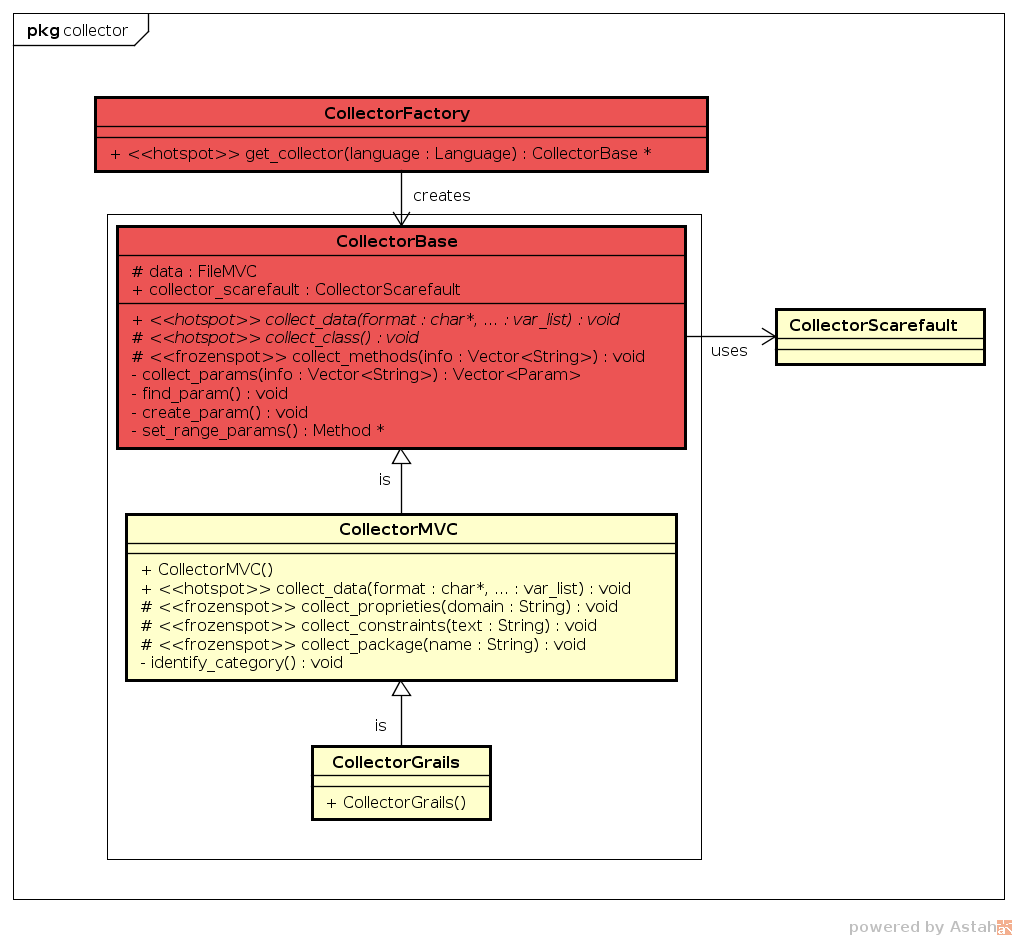
\includegraphics[width=\textwidth]{figuras/collector-grails-class-diagram.png}
    \caption{Diagrama de classes exemplificando a extensibilidade do \textit{factory pattern} no \framework}
    \label{collector-grails-class-diagram}
\end{figure}
\FloatBarrier

Na Figura \ref{collector-grails-class-diagram} observa-se que a classe
\lstinline|CollectorBase|, em vermelho, é o ponto de extensão. Como já descrito
na subseção \ref{subsec-factory-pattern}, há também uma classe, a \lstinline|CollectorMVC|,
já disponível para se estender, caso a linguagem alvo esteja acoplada
arquiteturalmente ao padrão de projeto MVC. Dessa forma, cria-se uma classe
derivada da \lstinline|CollectorMVC|, a \lstinline|CollectorGrails|.

Devido a essa herança, o \framework disponibiliza, à nova classe derivada,
alguns benefícios. Pela Figura \ref{collector-grails-class-diagram}, observa-se
que há algumas funções marcadas como \textit{hotspots} e outras como 
\textit{frozenspots}. Cabe a definição desses termos:

\begin{description}
\item[\textit{Frozenspots}:] são partes fixas do \textit{framework}. São as funções já
implementadas e que devem percamencer inalteradas. São comuns para qualquer linguagem alvo e auxiliam na adaptação do \textit{framework} para novas linguagens.
\item[	\textit{Hotspots}:] são as partes flexíveis do \textit{framework}. São nesses
pontos que há a extensão das funções do \textit{framework} por adição de
código, especificando a funcionalidade.
\end{description}

Assim sendo, a \lstinline|CollectorGrails| possui a mesma interface que a
sua classe mãe. O \framework abre como \textit{hotspot} a função
membro \lstinline|void collect_data(char *, ...)|, que é a única função membro
com escopo público. Qualquer classe que derive da \lstinline|CollectorBase| deve
implementar essa função. Não é diferente para a \lstinline|CollectorGrails|. No
entanto, ela é derivada da \lstinline|CollectorMVC|, que já implementa essa
função, de forma que a \lstinline|CollectorGrails| já está isenta de fazê-lo, mas
não proibida. Caso o desenvolvedor queira criar sua própria versão da
\lstinline|void collect_data(char *, ...)| ele pode criá-la. Para isso, ele conta
com algumas funções auxiliares já implementadas (\textit{frozenspots}), como a
\lstinline|void collect_methods(std::vector<std::string>)|.

Com a \lstinline|CollectorGrails| já implementada, pode-se utilizar outro
\textit{hotspot} do contexto da família dos \textit{collectors}: a
\lstinline|CollectorFactory|. A Figura \ref{collector-grails-class-diagram}
apresenta essa classe também como ponto de extensão, pois fazendo ajustes no
método \lstinline|CollectorBase * get_collector(Language)| estende-se sua
capacidade de seleção de coletores de dados. Um ajuste, nesse ponto, influencia
em qual coletor será escolhido dentro do \textit{parser}.

O Código \ref{get-collector-function} apresenta a alteração feita para estender
a \lstinline|CollectorBase * get_collector(Language)|.

\begin{lstlisting}[language=C++, label=get-collector-function, caption=Implementação e extensão da \lstinline{get_collector(Language)}]
CollectorBase * CollectorFactory::get_collector( Collector::Language language ) (*@\label{line:getcolletor-language}@*)
  {
    CollectorBase * instance;

    switch( language ) (*@\label{line:getcolletor-switch}@*)
    {
      case GRAILS:
        instance = new CollectorGrails(); (*@\label{line:getcollector-instancegrails}@*)
        break;
    }

    return instance; (*@\label{line:getcollector-return}@*)
  }
\end{lstlisting}

No Código \ref{get-collector-function}, a linha \ref{line:getcolletor-language}
mostra o cabeçalho da função. Nesse ponto, é importante ressaltar o uso como
parâmetro da enumeração \lstinline|Language|. Ela é definida no \lstinline|namespace|
\lstinline|Collector| para auxiliar o desenvolvedor. No caso exemplificado, foi
adicionado à enumeração a linguagem \textsf{Grails}. Na linha
\ref{line:getcolletor-switch}, usa-se um \lstinline|switch| para, a partir do parâmetro
\lstinline|language|, selecionar qual a linguagem. A linha
\ref{line:getcollector-instancegrails} faz a instanciação de um objeto do tipo
\lstinline|CollectorGrails| caso a linguagem seja orientada pela linguagem base do \textsf{Grails}. Para cada novo
coletor adicionado, um novo caso deve ser criado no \lstinline|switch|. Na linha
\ref{line:getcollector-return}, retorna-se a instância.

A Figura \ref{parser-instance-sequence-diagram} traz um diagrama de sequência para melhorar
visualização dos efeitos no \scarefault quando da instanciação de um objeto \lstinline|Parser|.
Essa visão é interessante para observar o comportamento esperado da
\lstinline|CollectorFactory|.
\begin{landscape}
\begin{figure}[h]
  \centering
    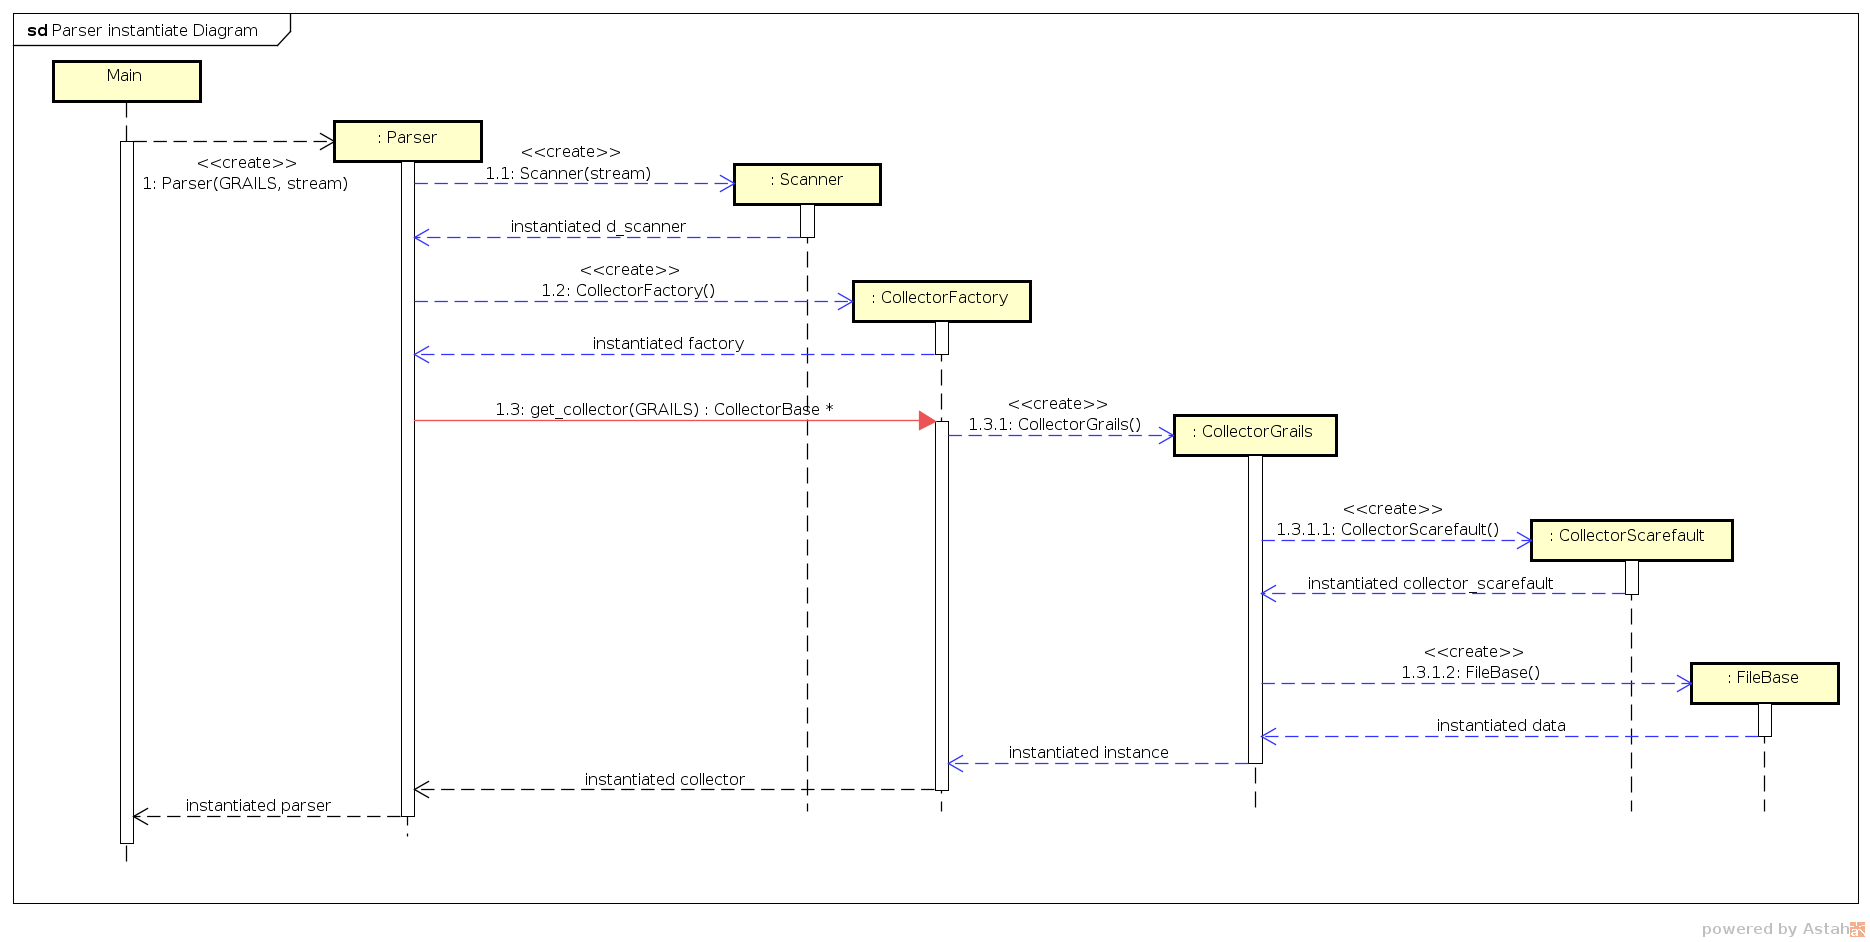
\includegraphics[width=1.5\textwidth]{figuras/parser-instance-sequence-diagram.png}
    \caption{Diagrama de sequência da instanciação de um \lstinline|Parser| e os efeitos na \lstinline|CollectorFactory|}
    \label{parser-instance-sequence-diagram}
\end{figure}
\FloatBarrier
\end{landscape}

A Figura \ref{parser-instance-sequence-diagram} mostra os objetos sendo
instanciados após a instância de um objeto \lstinline|Parser| ser solicitada.
A \lstinline|CollectorFactory|, recebendo como argumento a valor \textsf{Grails},
faz a instanciação de um objeto \lstinline|CollectorGrails| que, por sua vez,
traz consigo outros dois objetos importantes em sua formação: uma instância de um
\lstinline|CollectorScarefault|, que será responsável por extrair informações
dos comentátios de documentação, e um \lstinline|FileBase|, que mantém as informações
coletadas a partir do código fonte.

Nesse momento, o \lstinline|Parser| possui um agente de coleta de dados que atuará durante
o processamento do arquivo com o código fonte a ser testado. Devido à instanciação
no construtor do \lstinline|Parser|, é possível usá-lo no arquivo que contém as regras
gramaticais da linguagem alvo, nesse exemplo, a linguagem que orienta a programação na plataforma \textsf{Grails}. No Código
\ref{collector-in-use}, é possível observar como ocorre esse processo.

\begin{lstlisting}[language=C++, label=collector-in-use, caption=Agente coletor em uso no \parser]
[...]
untyped_method_stmt: (*@\label{line:collectoruse-noterminal}@*)
  DEF IDENTIFIER '(' param_list ')' { (*@\label{line:collectoruse-rule}@*)
    std::string identifier_token( (*@\textdollar@*)2 ); (*@\label{line:collectoruse-id-token}@*)
    std::string params_token( (*@\textdollar@*)4 ); (*@\label{line:collectoruse-param-token}@*)

    collector->collect_data( "mp", identifier_token.c_str(), params_token.c_str() ); (*@\label{line:collectoruse-collect-data}@*)
  }
;
[...]
\end{lstlisting}

No Código \ref{collector-in-use}, a linha \ref{line:collectoruse-noterminal}
apresenta a declaração de um novo símbolo não terminal da gramática, que é
definido pela regra gramatical ditada na linha \ref{line:collectoruse-rule}.
 Como pode ser observado, a regra ilustrada no exemplo, é a regra que rege a definição de métodos sem um tipo de retorno. As linhas \ref{line:collectoruse-id-token} e
\ref{line:collectoruse-param-token} atribuem a \textit{strings} os valores
identificados na segunda e na quarta posições da regra, identificadas pelos
\textit{tokens} \lstinline|INDETIFIER| e \lstinline|param_list|.

A linha \ref{line:collectoruse-collect-data} apresenta o uso do agente coletor
na definição da gramática. O operador \lstinline|->| é usado pois o objeto
\lstinline|collector| é um ponteiro ao agente coletor. A sintaxe de \cpp exige
que a referência a membros pertencentes a um objeto, a partir de um ponteiro, seja
feita por meio desse operador. A função \lstinline|void collect_data(char * format, ...)|
recebe como parâmetro uma \str em \textit{c-style} e uma quantidade ilimitada de
argumentos do tipo \str em \textit{c-style}. O primeiro parâmetro, \lstinline|format|, espera
uma \str que indique os tipos de dados que estão sendo coletados. A Tabela
\ref{reference-format-collect-data} apresenta uma referência ao tipo de dado e
o código a ser usado no parâmetro \lstinline|format|. No caso exemplificado,
o argumento é \lstinline|"mp"|, indicando a passagem do nome do método e a
lista de parâmetros desse método. Em seguida, são listados os dados a serem coletados.
Isso é feito passando os itens declarados nas linhas
\ref{line:collectoruse-id-token} e \ref{line:collectoruse-param-token}.

\begin{table}[h]
\centering
\caption{Descrição das letras identificadoras e o respectivo tipo de dado a ser coletado}
\label{reference-format-collect-data}
\begin{tabular}{@{}cc@{}}
\toprule
\textbf{Letra Identificadora} & \textbf{Tipo de Dado}        \\ \toprule
P                             & Pacote                       \\ \hline
c                             & Classe                       \\ \hline
m                             & Método                       \\ \hline
p                             & Lista de Parâmetros          \\ \hline
\end{tabular}
\end{table}

É importante ressaltar que, embora já haja uma versão disponível da
\lstinline|collect_data(char *, ...)| para as classes derivadas da
\lstinline|CollectorMVC|, pode-se sobreescrevê-la. A Tabela
\ref{reference-format-collect-data} é relativa à versão já disponibilizada
pelo \textit{framework}. No caso, preferiu-se utilizar a já disponível.

Ao utilizar a função \lstinline|void collect_data(char *, ...)|, uma série
de chamadas a outras funções é feita. A Figura \ref{collect-data-sequence-diagram}
apresenta a dinâmica desse processo.
\begin{landscape}
\begin{figure}[h]
  \centering
    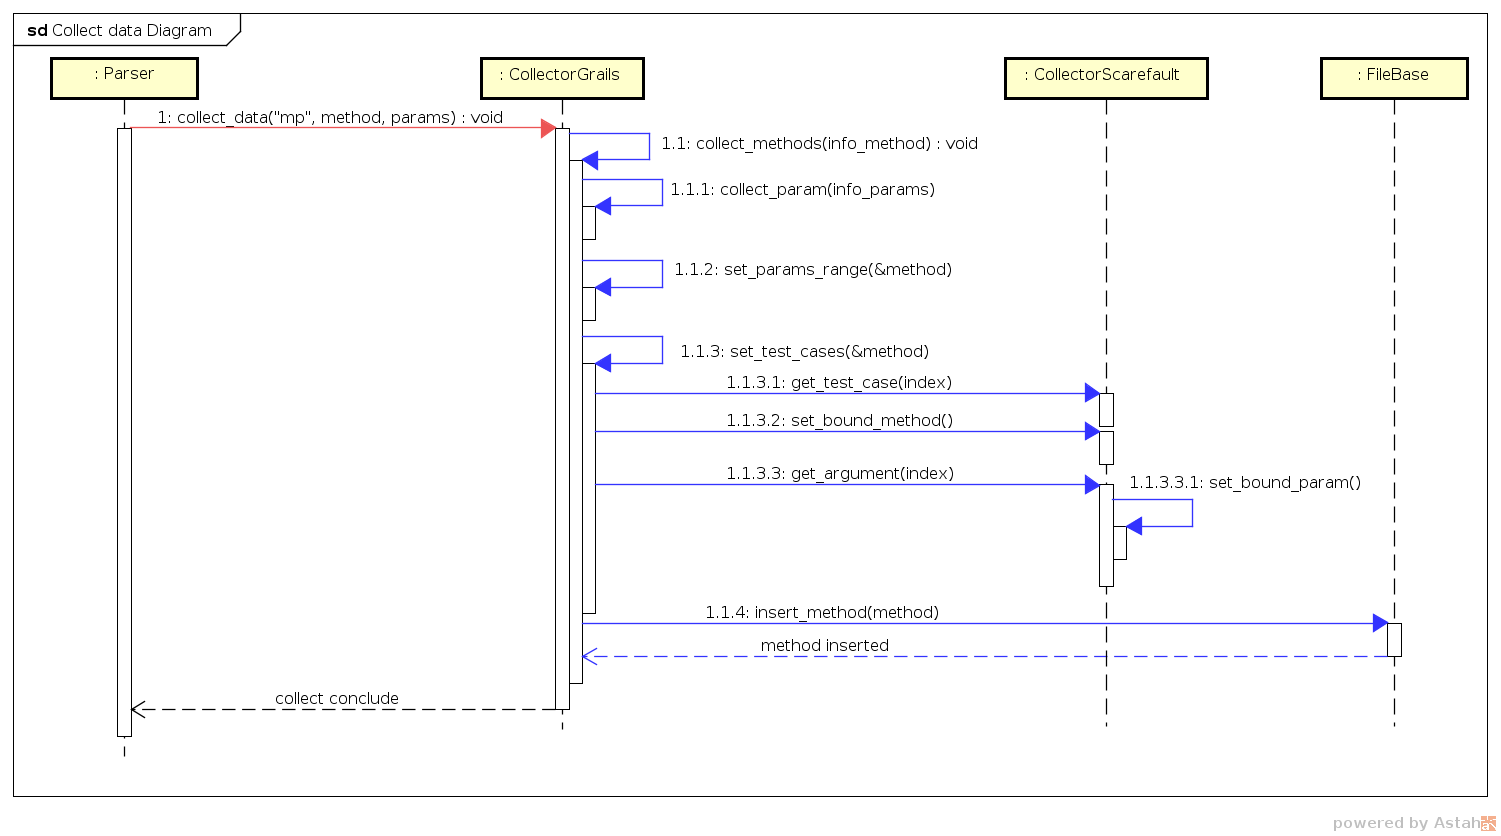
\includegraphics[width=1.5\textwidth]{figuras/collect-data-sequence-diagram.png}
    \caption{Diagrama de sequência das chamadas de funções por trás da \lstinline|void collect_data(char *, ...)|}
    \label{collect-data-sequence-diagram}
\end{figure}
\FloatBarrier
\end{landscape}

Nesse diagrama, houve a diferenciação da ação tomada por um \textit{hotspot}, em vermelho, e um \textit{frozenspot}, em azul. É possível verificar que o \lstinline|void collect_data(char *, ...)| realiza a coleta dos dados em etapas. Inicialmente, é coletado as informações do método, sendo elas o nome do método e nome e tipo da lista de parâmetros. Em seguida, são definidos parâmetros de teste conforme o intervalo solicitado no código-fonte, caso haja. São criados, então, os casos de testes baseado nas informações coletadas, relaciona-os com o método identificado. Por fim, os casos de testes são inseridos no \lstinline|FileMVC|, e ocorre a conclusão da coleta dos dados desse método.

Com isso, a primeira parte para o uso do \scarefault está finalizada, ou seja, o \textit{framework} está preparado para coleta de dados. A segunda etapa é responsável pela produção dos casos de teste.

\subsubsubsection{Criação do agente de construção de casos de teste}
Com os dados essenciais para os testes já coletados por um
\lstinline|CollectorBase| e armazenados em um \lstinline|FileBase|,
faz-se necessária a criação de um agente responsável pela
produção do arquivo de teste. Para isso, o \framework disponibiliza como
ponto de extensão a classe \lstinline|TestfileBuilder|. Como já explicitado
na Figura \ref{testfile-diagram}, ela faz parte de um conjunto de classes
que seguem o \textit{Builder Pattern}. Esse padrão permite separar a criação
de objetos complexos em dois elementos: a sua representação e o processo de
criação. Arquivos de teste são elementos, que têm estruturas diferentes, conforme
a linguagem de programação, mas o processo de construção é semelhante.

Retomando a Figura \ref{testfile-diagram}, na qual é apresentada a
estrutura do \textit{Builder Pattern} no projeto, para o caso de exemplo
com o \grails o diagrama de classes passa a ser o exposto na Figura
\ref{testfile-grails-class-diagram}.

\begin{figure}[h]
  \centering
    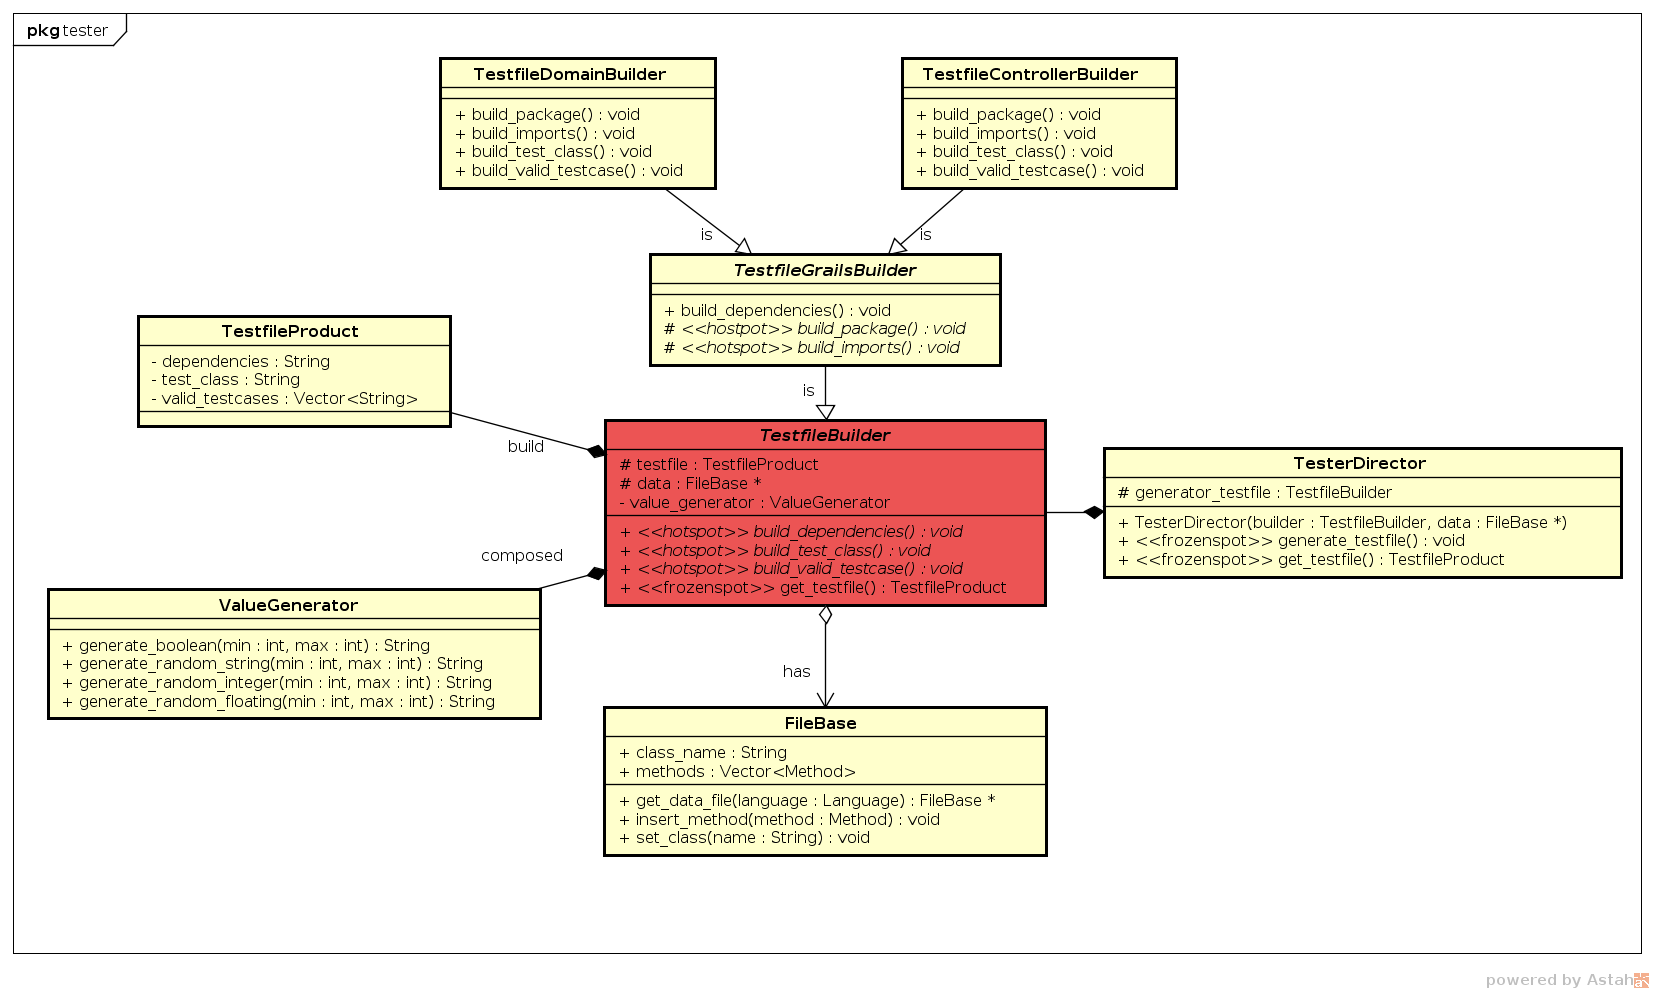
\includegraphics[width=\textwidth]{figuras/testfile-grails-class-diagram.png}
    \caption{Diagrama de classes exemplificando a extensibilidade do \textit{builder pattern} no \framework}
    \label{testfile-grails-class-diagram}
\end{figure}
\FloatBarrier

Na Figura \ref{testfile-grails-class-diagram}, destaca-se em vermelho
o ponto de extensão: a classe \textsf{TestfileBuilder}. Essa classe é responsável
pela construção do objeto \lstinline|testfile|, pertencente à classe
\lstinline|TestfileProduct|. Essa classe possui três \textit{hotspots} para adaptação, as funções
\lstinline|void build_dependencies()|, \lstinline|void build_class()| e
\lstinline|void build_validtestcase()|. Qualquer classe derivada a partir dessa classe é
obrigada a implementar sua própria versão dessas funções. Isso permite a extensão
do \framework e garante que o desenvolvedor seguirá as regras para a construção do
\lstinline|TestfileProduct| pelo processo comum. No caso de exemplo com o
\textsf{Grails}, criou-se a classe \lstinline|TestfileGrailsBuilder|. Com base
nessa classe, surgem outras duas: \lstinline|TestfileControllerBuilder| e
\lstinline|TestfileDomainBuilder|. A classe \lstinline|TestfileGrailsBuilder|
implementa a \lstinline|void build_dependencies()|, mas passa a responsabilidade
para as suas classes derivadas de implementar outras duas funções: a
\lstinline|void build_package()| e a \lstinline|void build_imports()|. Assim,
as classes \lstinline|TestfileControllerBuilder| e \lstinline|TestfileDomainBuilder|
são responsáveis por implementar as quatro funções exigidas no processo
construção de arquivos de teste para \textsf{Grails}. Essas duas classes exigem, pois testes de controller configuram-se de forma
distinta de testes feitos para \textit{models}. Assim, optou-se por realizar duas classes
diferentes para esses dois tipos de arquivos.

Tendo o \textit{Builder Pattern} extendido pode-se usar o\textit{framework}.
O Código \ref{testfile-in-use} apresenta um exemplo de \lstinline|main| para
o uso do \Scarefault.

\begin{lstlisting}[language=C++, label=testfile-in-use, caption=Agente testador sendo usado na função \lstinline|main|]
#define ACCEPTABLE_QTD_ARGS 3 (*@\label{line:testfileuse-qtd-args}@*)
#define SOURCE_FILE_NAME 2 (*@\label{line:testfileuse-filename}@*)
#define OPTION 1 (*@\label{line:testfileuse-option}@*)
#define TYPE_TEST 3 (*@\label{line:testfileuse-typetest}@*)
[...]
if( !strcmp( argv[ OPTION ], "generate" ) ) (*@\label{line:testfileuse-ifoption}@*)
{
  if( !strcmp( argv[ TYPE_TEST ], "controller" ) ) (*@\label{line:testfileuse-iftype}@*)
  {
    TesterDirector tester( new TestfileControllerBuilder( collector_ptr->get_data() ) ); (*@\label{line:testfileuse-directorcontroller}@*)
    tester.generate_testfile(); (*@\label{line:testfileuse-generate-c-testfile}@*)

    Writer writer( &tester, argv[ SOURCE_FILE_NAME ] ); (*@\label{line:testfileuse-writer-c}@*)
    writer.write_testfile(); (*@\label{line:testfileuse-write-c-testfile}@*)
  } else if( !strcmp( argv[ TYPE_TEST ], "domain" ) ) (*@\label{line:testfileuse-elsetype}@*)
  {
    TesterDirector tester( new TestfileDomainBuilder( collector_ptr->get_data() ) ); (*@\label{line:testfileuse-directordomain}@*)
    tester.generate_testfile(); (*@\label{line:testfileuse-generate-d-testfile}@*)

    Writer writer( &tester, argv[ SOURCE_FILE_NAME ] ); (*@\label{line:testfileuse-writer-d}@*)
    writer.write_testfile(); (*@\label{line:testfileuse-write-d-testfile}@*)
  }
}
[...]
\end{lstlisting}

No Código \ref{testfile-in-use}, a linha \ref{line:testfileuse-ifoption}
faz a comparação da opção passada pela linha de comando, sendo que a palavra
\textit{generate} entra no bloco de instruções. As linhas
\ref{line:testfileuse-iftype} e \ref{line:testfileuse-elsetype} fazem a
comparação da \str passada na linha de comando: caso seja igual a
\textit{controller}, executa um trecho de código específico. Se for \textit{domain}, executa outro trecho de código. As linhas \ref{line:testfileuse-directorcontroller} e
\ref{line:testfileuse-directordomain} explicitam a instanciação de um
objeto da classe \lstinline|TestfileDirector|. Esse objeto exige no
seu construtor a passagem de um objeto do tipo \lstinline|TestfileBuilder|,
que por sua vez exige um \lstinline|FileBase| para trabalhar os dados. Essa
é a forma de trabalho do \textit{Builder Pattern}: o \lstinline|TesterDirector|
mantém o processo de construção do arquivo de teste, requisitando apenas o
tipo de representação que deve ser construída. Isso é revelado por meio do
tipo de \textit{builder} passado como argumento. As linhas
\ref{line:testfileuse-generate-c-testfile} e \ref{line:testfileuse-generate-d-testfile}
chamam a função que constrói o arquivo de teste.


As linhas \ref{line:testfileuse-writer-c} e \ref{line:testfileuse-writer-d}
instanciam um objeto do tipo \lstinline|Writer|. Ele é responsável por escrever
o arquivo de teste gerado pelo \lstinline|TesterDirector|. Para isso, ele
recebe o objeto \lstinline|TesterDirector| e o nome do arquivo fonte.

Para melhor visualizar a dinâmica do funcionamento por trás do Código
\ref{testfile-in-use}, a Figura \ref{generate-testfile-sequence-diagram}
traz um diagrama de sequência que reflete esse funcionamento.

\begin{landscape}
\begin{figure}[h]
  \centering
    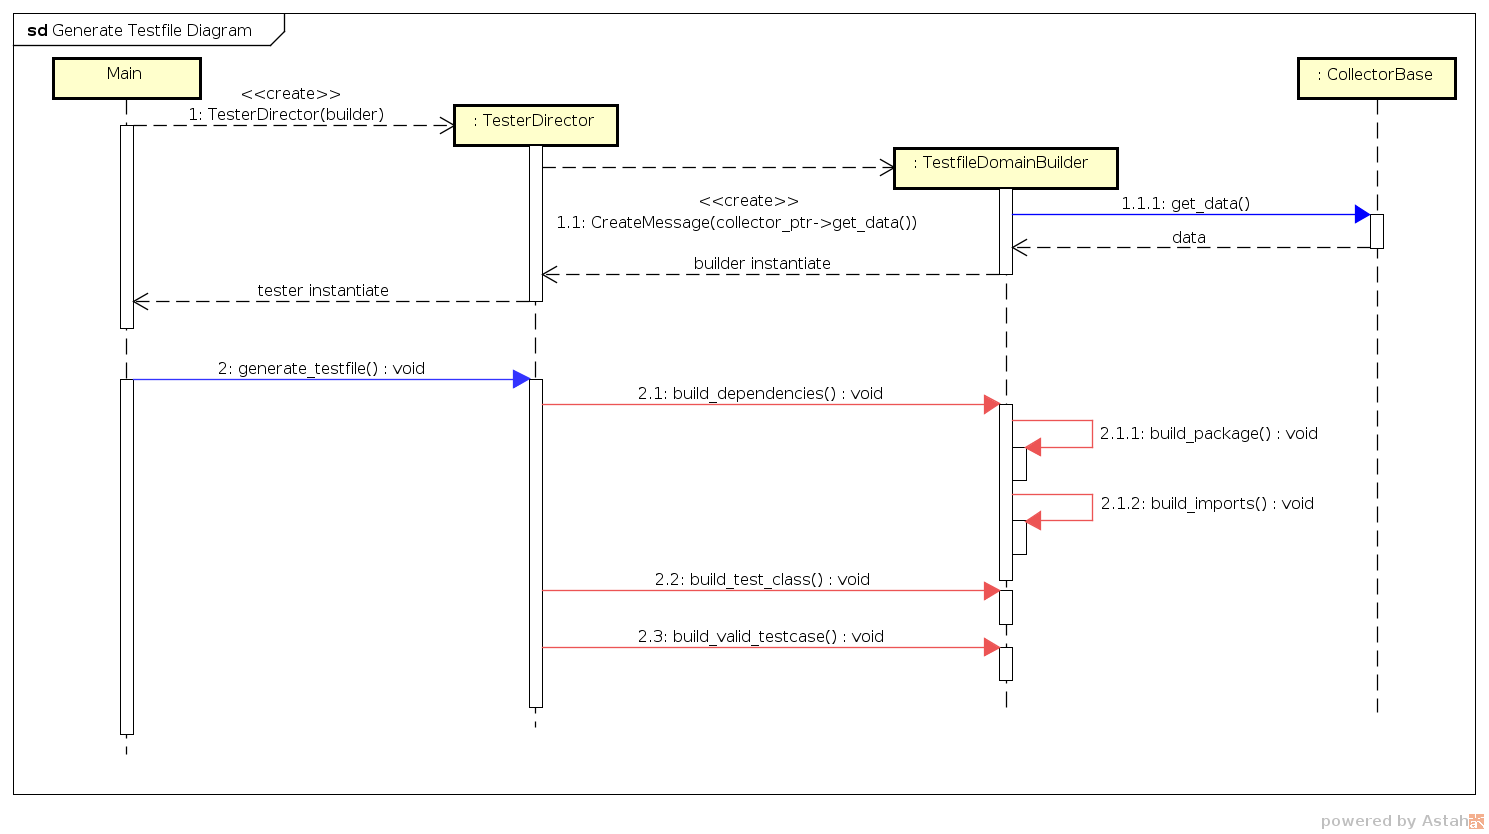
\includegraphics[width=1.5\textwidth]{figuras/generate-testfile-sequence-diagram.png}
    \caption{Diagrama de sequência das chamadas de funções por trás da \lstinline|void generate_testfile()|}
    \label{generate-testfile-sequence-diagram}
\end{figure}
\FloatBarrier
\end{landscape}

O diagrama na Figura \ref{generate-testfile-sequence-diagram} mostra a instanciação
de um objeto do tipo \textsf{TesterDirector} Para o exemplo, foi selecionado
o caso em que a representação para o \lstinline|testfile| é de uma
\textit{domain}. Assim sendo, é passado como argumento para o construtor do
\lstinline|testerDirector| uma nova instância de \lstinline|TesterDomainBuilder|,
que por sua vez exige no seu construtor um objeto do tipo \lstinline|FileBase|.
Este é passado através da chamada da função \lstinline|get_data()| do
\lstinline|CollectorBase|. Assim, o \lstinline|TesterDirector| é instanciado.

Na segunda parte do diagrama de sequência, observa-se a chamada da função
\lstinline|void generate_testfile()|. A cor azul indica que ela é um
\textit{frozenspot}. Ela carrega o processo de construção de um
arquivo de teste. Para isso, ele faz a chamada dos passos de construção,
implementados pelo \lstinline|TestfileDomainBuilder|. Vale lembrar que
todas as funções chamadas após a \lstinline|void generate_testfile()| são
hotspots, em vermelho. O diagrama da Figura \ref{generate-testfile-sequence-diagram}
é interessante, pois evidencia bem o \textit{hollywood principle}: o
desenvolvedor não faz a chamada ao \textit{framework}. É o \framework que chama
as funções criadas pelo desenvolvedor.

\subsection{Geração de Testes Unitários}
Além da utilização do \scarefault como \textit{framework}, pode-se usá-lo como
aplicação, após às devidas adaptações por parte dos desenvolvedores. Supondo
que o \scarefault já tenha sido adaptado para  \textsf{Grails}, o alvo inicial
desse projeto, segue um exemplo de como utilizar o \scarefault como uma
aplicação.

A geração de testes unitários feita pelo \scarefault é dada em duas etapas:
na primeira é solicitada a criação de casos de teste ao \Scarefault. Isso
quer dizer que o \scarefault vai gerar, a partir de determinados parâmetros
expostos pelo usuário, casos de teste. Na segunda etapa, é requisitada a
geração dos testes definidos como casos de teste, completados com informações
adicionais pelo usuário.

Para a demonstração, foi criado uma função \lstinline|main|. Por meio dessa
função, é possível a chamada do \scarefault e seus benefícios por linha
de comando. Segue o Código \ref{generic-call-scarefault} que traz um
\textit{template} de chamada do \Scarefault.

\begin{lstlisting}[language=bash, label=generic-call-scarefault, caption=Template para chamada do \scarefault pela linha de comando]
(*@\textdollar@*) ./scarefault <opção> <caminho ao arquivo a ser testado> [categoria do padrão MVC]
\end{lstlisting}

O argumento referenciado como \lstinline|<opção>| indica qual a opção que o
usuário escolheu. Essa \lstinline|<opção>| pode variar entre \lstinline|create|
e \lstinline|generate|.
\begin{description}
\item[\textsf{create}:] opção que solicita ao \scarefault a criação de
casos de teste. Isso é efetuado através da leitura de alguns dados
diponibilizados pelo usuário dentro dos comentários de documentação dos
métodos.
\item[\textsf{generate}:] opção que requisita ao \scarefault a geração
dos testes, baseando nos casos de teste criados anteriormente. Os casos de
teste criados pela opção \lstinline|create| devem ser completados com o
valor esperado pelo teste. O usuário também pode acrescentar casos de testes, caso sejam necessários, seguindo, seguindo o padrão proposto pelo \Scarefault.
\end{description}

O argumento referenciado como \lstinline|<caminho ao arquivo a ser testado>|
deve ser preenchido com o caminho que leva até o arquivo com o código fonte
a ser testado. O argumento referenciado como \lstinline|[categoria do padrão MVC]|
deve ser preenchido ou com \lstinline|controller| ou com \lstinline|domain|.

Considerando-se o que foi dito, toma-se o arquivo \textsf{domain.groovy} como
exemplo. Ele contém o Código \ref{domain-groovy}.
\begin{lstlisting}[language=C++, label=domain-groovy, caption=Código do arquivo domain.groovy]
package math

class Math {
  def sumTwoNumbers(int parcel1, int parcel2) {
    def total = parcel1 + parcel2
    return total
  }
}
\end{lstlisting}

O usuário do \scarefault deve adicionar ao Código \ref{domain-groovy} comentários
de documentação contendo algumas marcações próprias do \Scarefault.
Essas marcações são referenciadas pela Tabela \ref{scarefault-marks}.

\begin{table}[h]
\centering
\caption{Marcações de comentários para uso do \scarefault}
\label{scarefault-marks}
\begin{tabular}{@{}cc@{}}
\toprule
Marcação           & Descrição                                                                                                                                                                \\ \toprule
\textsf{@param}  & Indica para o \textsf{Scarefault} o nome do parâmetro                                                                                                                  \\ \hline
\textsf{@range}  & Indica para o \textsf{Scarefault} os valores limites relativos ao parâmetro                                                                                            \\ \hline
\textsf{@test}   & \begin{tabular}[c]{@{}c@{}}Indica para o \textsf{Scarefault} os argumentos que devem ser passados\\ ao método durante o teste. Evidência um caso de teste\end{tabular} \\ \hline
\textsf{@expect} & Indica para o \textsf{Scarefault} o valor esperado no caso de teste                                                                                                    \\ \hline
\end{tabular}
\end{table}

Assim, com a adição do comentário de documentação, o Código \ref{domain-groovy}
passa a ficar como o Código \ref{domain-groovy-doc}.
\begin{lstlisting}[language=C++, label=domain-groovy-doc, caption=Código do arquivo domain.groovy com as marcações do \scarefault]
package math

class Math {
  /**
    @param parcel1 @range 0..100 (*@\label{line:domaingroovy-param1}@*)
    @param parcel2 @range 0..100 (*@\label{line:domaingroovy-param2}@*)
  */
  def sumTwoNumbers(int parcel1, int parcel2) {
    def total = parcel1 + parcel2
    return total
  }
}
\end{lstlisting}

O usuário então solicita ao \scarefault a criação dos casos de teste.
Isso se dá pela linha de comando:
\lstinline|./scareafault create domain.groovy|. Assim,
o código passa a ficar como o Código \ref{domain-groovy-testcase}.
\begin{lstlisting}[language=C++, label=domain-groovy-testcase, caption=Código do arquivo domain.groovy com os casos de teste]
package math

class Math {
  /**
    @param parcel1 @range 0..100 (*@\label{line:domaingroovy-param1}@*)
    @param parcel2 @range 0..100 (*@\label{line:domaingroovy-param2}@*)
    @test (0, 50) @expect INSERT_HERE
    @test (1, 50) @expect INSERT_HERE
    @test (99, 50) @expect INSERT_HERE
    @test (100, 50) @expect INSERT_HERE
    @test (50, 0) @expect INSERT_HERE
    @test (0, 1) @expect INSERT_HERE
    @test (0, 99) @expect INSERT_HERE
    @test (0, 100) @expect INSERT_HERE
  */
  def sumTwoNumbers(int parcel1, int parcel2) {
    def total = parcel1 + parcel2
    return total
  }
}
\end{lstlisting}

O usuário então deve inserir as expectativas dele para cada caso
de teste e, em seguida, executar a linha de comando:
\lstinline|./scareafault generate domain.groovy domain|.
Dessa forma, o \scarefault gera os testes especificados em um outro
arquivo, chamado de \lstinline|domainTests.groovy| no mesmo diretório
do \lstinline|domain.groovy|.

\section{Resumo do Capítulo}
  Este capítulo detalho o produto final desse trabalho: o \Scarefault. Abordou-se incialmente uma visão geral, seguindo da análise da arquitetura e, por fim, a utilização do \textit{framework}.